\documentclass[../dissertation.tex]{subfiles}

\begin{document}

\section{Robotics Overview}
\label{background-robotics}

Robotics is the study of autonomous computer systems, usually involving physical interaction with it's environment. Robotics lies at the intersection between computing science, eletrical and mechanical engineering. Robotics has been common in popular culture since the 1940s\cite{hockstein2007history}, but due to the speed of technological growth, has quickly become widely ingrained in many industries. The first industrial use of robotics was in manufacturing, with General Motors putting the first robot into service in 1961\cite{hagele2016ashorthistory}. Nowadays, with great increases in computing power, sensor accuracy, research investment, and software algorithms, example applications of robotics include manufacturing, agriculture, construction, mining, disaster recovery, medicine, health care, and surveillance\cite{hagele2016robotsatwork}.

Today's robotic systems generally consist of many small autonomous systems working together to form a coherent whole\cite{4058987}. For example, a particular sensor (say a camera) may be constantly recording data and storing it in some buffer (erasing the oldest when full). This subsystem does not depend on any others to complete its task (recording the environment), but other subsystems may rely on its output (such as a computer vision package which needs video frame inputs). This style of robot design is becoming increasingly prevelant, with many robotic middlewares adopting this distributed approach.

Robotics is related to a field called cyber-physical systems (CPS) that concerns integrating computer systems with the physical world\cite{Lee:EECS-2008-8}. These can include Internet Of Things (IoT) networks\cite{atzori2010internet} which can (for example) be used to control things around the household, such as light switches, central heating systems, and hoovering. This is distinct from robotics as CPS generally embody a `think globally, act locally' approach\cite{gordonthink} (such as using data from many sources to improve the CPS' performance in each), compared to robotics which utilises a more `think locally, act locally' strategy - meaning that each instance of a robot generally makes it's own decisions, and acts upon them solely.

This chapter aims to provide the background knowledge required to understand the significance of the results presented in this paper. Section \ref{section-multi-robot-systems} discusses the concept of multi-robot systems, as well as their application in society. Section \ref{background-scalability} outlines what scaling refers to in the context of a robotic system. Next, Section \ref{robotic-middleware} introduces robotic middleware, and why it is useful when constructing a robotic system. This section also presents a tabular overview of a range of common robot middlewares, and discusses the main concepts seen in many middlewares. Section \ref{background-ros} then outlines the architecture of ROS, which is the middleware of particular study in this paper. Finally, Section \ref{background-robot-config} discusses the configuration of the robot car kit platform used in later experiments.

\section{Multi-Robot Systems}
\label{section-multi-robot-systems}

Multi-robot systems are specific instances of mult-agent systems. They represent a joint problem space between robotics, artificial intelligence, and distributed systems. Multi-robot systems as a formal concept is a recent development with a IEEE technical committee only being formed in 2014\cite{MultiRobotSystemsIEEECommittee}.

Multi-robot systems can consist of many intelligent agents (each of which may be comprised of many small autonomous systems) working to solve a task that any one system may not be able to solve alone. These multi-robot are distinct from a multi-agent system in which individual nodes are generally stationary, as each agent in a multi-robot system is mobile\cite{doi:10.5772/57313}. Mobile robotics has been made more possible recently by advances in battery\cite{estrin2002connecting} and wireless communication\cite{cordeiro2010ieee} technologies. One such application of a multi-robot (and mobile) system is warehouse automation. Hamberg (2012)\cite{hamberg2012automation} provides a comprehensive overview of such a system, but a brief description is provided below.

In a warehouse, millions of items can be spread throughout miles of shelving and the requirement is that a random subset of items (those that have been bought) must arrive at a specific point (the delivery pick-up point) at a specific time (when the van is there). This task previously could be solved by having human pickers wander the isles searching for items - however given recent increases in the size of online shopping this is no longer feasible. Now, online retailers (such as Amazon) are using hundreds of individual robots to intelligently move the shelving around and bring the correct items to stationary human pickers\cite{wurman2008coordinating}. This system requires the coordination of the individual robots, but they must all act independently in order to efficiently keep pace with the items ordered. However, this system still requires human pickers to lift items off the shelves, and place them in boxes. Amazon is using competitions such as the Amazon Picking Challenge to encourage researchers to develop reliable methods to automate this picking task\cite{correll2016lessons}, although we have still not reached the level of full automation in a production environment.

\section{Scalability in Robotics}
\label{background-scalability}

When creating multi-robot systems, scalability becomes an important concern\cite{klavins2004communication}. It is a crucial decision for a system architect to choose between using a small number of expensive highly-powered robot systems and using a larger number of simpler, cheaper robot systems to improve overall system performance. There are several factors to consider include the processing power of each robot, the communication framework required to organise them, the cost of each robot, and the suitability of the problem to a multi-robot system.

Scalability can refer to many different concepts. Some define it as the ability to handle more code, others as more processes, and yet others as more hardware\cite{Bondi:2000:CSI:350391.350432}. This paper will consider the latter two definitions, and will refer to increasing the number of processes running on the same amount of hardware as `vertical' scaling, and increasing the amount of hardware (e.g. number of host machines) as `horizontal' scaling. There are a number of advantages and disadvantages to both.

Vertical scaling is useful if a single instance of the process (or node) does not saturate any of the resources of the host machine - for example, a single threaded computation-heavy application running a multi-core processor architecture. There are still other CPU cores available to run more instances of the application, with the benefit of gaining higher throughput. However, if a single instance does saturate a resource (e.g. high RAM usage, full disk usage, or network saturation) then vertical scaling will introduce resource contention problems, such as two disk IO (input-output) heavy processes competing for disk access and thus slowing both down. Extreme vertical scaling will also cause problems with context switching in the processor. If thousands of processes are competing to get time on the processor, then the process scheduler will only schedule each process for a very short timeslice before switching in a new process. This can introduce an overhead due to the time taken to switch out a running process, and switch in a new process.

Horizontal scaling alleviates some of the problems with vertical scaling. By scaling nodes over multiple hosts, each host has access to a completely independent set of resources (e.g. it's own CPU, RAM, disk, and GPU) - this reduces resource contention issues. However, horizontal scaling introduces a number of complex issues, such as the requirement for managing an increasing amount of hardware - all disks fail eventually and must be replaced, and increasing the total number of disks in the system results in an increased number of failures, requiring replacements to be fitted more often. For this reason, horizontally scaled (or distributed) systems must be more fault-tolerant than single host systems. Increasing the number of hosts also has implications for the monetary cost of the system, as duplicating hardware also duplicates costs (such as initial purchase, maintenance, and running costs). Swarm robotics is the extreme approach of horizontal scaling, involving creating many very simple robots which individually could not solve tasks or survive environments - however when they work together as a form of society they can work efficiently\cite{csahin2004swarm}.

\section{Robotic Middleware}
\label{robotic-middleware}

As mentioned previously in Section \ref{background-robotics}, software for robots is generally written as a collection of autonomous subsystems, often called modules. Robotic middleware is a software infrastructure that is intended to provide convenient abstraction and communication paradigms for facilitating this multi-subsystem approach. In general, a robotics middleware would provide interfaces for defining each subsystem, and defining how each subsystem communicates with others. A specific example is the Player Project. Player provides an abstraction layer for robotic coding, which lets developers focus more on their specific application logic, rather than boilerplate communication code\cite{vaughan2003device}. The different approaches of specific middlewares is discussed later in Section \ref{overview-of-robotic-middleware}.

A typical robot may consist of many individual sensors, for example a camera that can record 720p (a resolution of 1280x720) RGB video at 30fps (frames-per-second), a LIDAR range sensor that can measure distances of up to 30m at a frequency of 1-500Hz, a tri-axis gyroscope and accelerometer capable of measuring up to 16g of force with a measurement frequency of 40Hz. These devices use a range of sophisticated technologies to measure and analyse the physical world, each recording a different data format at a different data rate. Figure \ref{pr2-diagram} shows the sensors available on Willow Garage's PR2 robot. These sensor modules are all independently designed, resulting in a wide array of different software and hardware interfaces - meaning that each robot software developer that wishes to use these sensors must create the software to communicate with these sensors, consume their data, and then write the robotic software that makes use of it. This results in a wide variety of implementations for manipulating the same data on each sensor, increasing the likelihood of implementation mistakes, misunderstandings, and wasting researchers' time.

\begin{figure}[H]
\centering

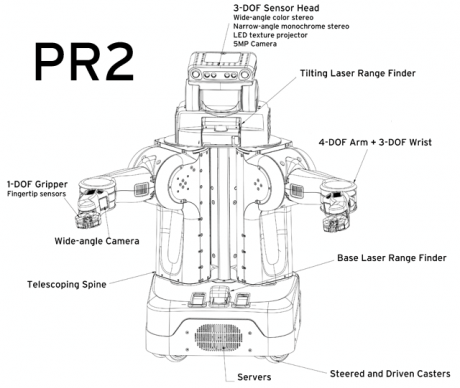
\includegraphics[width=0.7\textwidth]{images/background/Williow-Garage-PR2-Drawing-Diagram.png}
\caption{Diagram outlining the major sensors present on Willow Garage's ROS-powered PR2 robot\cite{pr2OverviewDiagram}}
\label{pr2-diagram}
\end{figure}

Robotic middleware is the solution to this problem. A middleware provides a common interface design so that no matter what hardware is producing the data, the results are distributed in a consistent manner. This means that hardware manufacturers (or users) need only to implement one software system for each sensor that can then be distributed and reused amongst all users of that sensor, as long as those users are using that middleware. This means that creators of a  system utilising the same middleware have easy access to the data created by a particular sensor as they know the software they create will be able to easily consume the sensor's data stream.

Another benefit of middleware is that this communication interface can be reused within the robotic system for communicating between distinct modules within the system. For example, a robot software developer may create a computer vision module that processes a video stream and returns a data stream containing a description of the objects in the video stream at each frame. When utilising a middleware, the researcher can make the result of their computer vision module available in a similar fashion to the sensor's video stream - meaning that high level software can utilise the results as if there was an `object-detecting hardware sensor'. These levels of abstractions make software much more maintainable, and reusable.

\end{document}
